\newcommand{\ScenarioA}{
\begin{tabular}{lrrr}\toprule Policy & Expected doses & km & Objective\\\midrule
static linear & 1614.7 & 78.9 & 1535.8\\
embedded linear & 1614.7 & 78.9 & 1535.8\\
static MLP & 1541.0 & 73.1 & 1467.9\\
embedded MLP & 1614.7 & 78.9 & 1535.8\\
historical mean & 1614.7 & 78.9 & 1535.8\\
benchmark & 1614.7 & 78.9 & 1535.8\\
\bottomrule\end{tabular}
\par\vspace{2mm}{\small Benchmark optimum interval: [1535.83, 1536.23]}
}
\newcommand{\ScenarioB}{
\begin{tabular}{lrrr}\toprule Policy & Expected doses & km & Objective\\\midrule
static linear & 1883.0 & 62.2 & 1820.8\\
embedded linear & 1883.0 & 55.7 & 1827.3\\
static MLP & 1883.6 & 74.1 & 1809.5\\
embedded MLP & 1875.4 & 52.5 & 1822.9\\
historical mean & 1883.5 & 55.5 & 1828.0\\
benchmark & 1880.5 & 51.8 & 1828.7\\
\bottomrule\end{tabular}
\par\vspace{2mm}{\small Benchmark optimum interval: [1828.69, 1829.18]}
}
\newcommand{\TrainingExample}{
\begin{tabular}{rrrrr}\toprule $\log$ pop & Unvaccinated & Accessibility & Exposure & Served\\\midrule
10.42 & 0.36 & 0.48 & 0.00 & 237.27\\
10.79 & 0.41 & 0.60 & 0.00 & 250.00\\
10.32 & 0.49 & 1.00 & 0.00 & 250.00\\
\bottomrule\end{tabular}
}
\newcommand{\RunEnvironment}{
11th Gen Intel(R) Core(TM) i7-1185G7 @ 3.00GHz\\[2mm]4 cores, 8 logical processors; 63.7 GiB RAM.\\[2mm]Windows-11-10.0.26200-SP0; Python 3.12.14; Gurobi 13.0.3.\\[2mm]scikit-learn 1.9.1; gurobi-machinelearning 1.7.0.\\[2mm]2 solver threads; 60 s limit; relative MIP gap 1e-06.\\[2mm]Run: 2026-09-29T09:02:56 UTC; full versions, seeds and hashes in results/environment.json.
}

\begin{frame}[plain,noframenumbering]
  \titlepage
\end{frame}

\begin{frame}{A forecast can change when the plan changes}
  \begin{itemize}
    \item A mobile clinic chooses which wards to serve and how to travel between them.
    \item Visits nearby may reduce demand through cannibalisation or increase it through mobilisation.
    \item A demand forecast fixed before routing can miss this dependence.
  \end{itemize}
  \vspace{4mm}
  \begin{block}{Today's question}
    What changes when the same predictor becomes a constraint inside the routing model?
  \end{block}
  \vspace{2mm}
  \small A synthetic teaching companion to Mayukh Ghosh's Chapter 6, with Chintan Amrit and Joaquim Gromicho. The outcomes shown here are simulated.
\end{frame}

\begin{frame}{One county, twenty candidate service points}
  \begin{columns}
    \begin{column}{.47\textwidth}
      \begin{itemize}
        \item Nyamira County, Kenya.
        \item Ward centroids snapped to an OSM drive network.
        \item An open path from Township, with at most eight serviced wards.
        \item The teaching depot also receives service and counts as a stop.
      \end{itemize}
      \vspace{2mm}
      \small Actual clinic sites and the referral hospital's coordinates would be needed for operational use.
    \end{column}
    \begin{column}{.53\textwidth}
      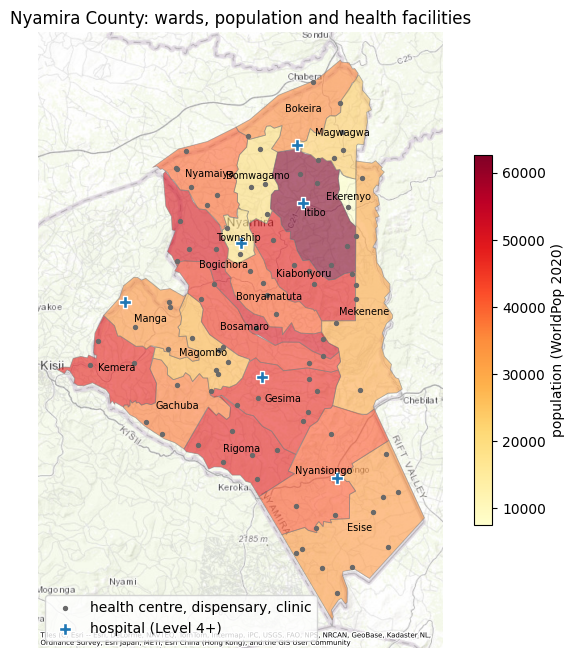
\includegraphics[width=\textwidth,height=.73\textheight,keepaspectratio]{figs/map.png}
    \end{column}
  \end{columns}
\end{frame}

\begin{frame}{Data sources and what they establish}
  \small
  \begin{tabular}{p{.25\textwidth}p{.67\textwidth}}
    \toprule
    Boundaries & GADM 4.1. Downloaded for local academic use; boundary files are not redistributed.\\[2mm]
    Population & WorldPop 2020, 1 km, UN-adjusted.\\[2mm]
    Roads & OpenStreetMap contributors; directed shortest-path distances through Pandana.\\[2mm]
    Facilities & Maina et al. (2019), 98 historical records; six hospital labels used as an accessibility proxy.\\[2mm]
    Outcomes & Synthetic unvaccinated shares, demand and spillovers.\\
    \bottomrule
  \end{tabular}\par
  \vspace{3mm}
  Hospital labels do not verify cold-chain capability. The county filter excludes facilities outside Nyamira.\par
  \vspace{2mm}
  \weblink{https://github.com/gromicho/mobile_clinics/blob/main/DATA_SOURCES.md}{Sources, licences and provenance}
\end{frame}

\begin{frame}{Facility selection changes the accessibility proxy}
  \centering
  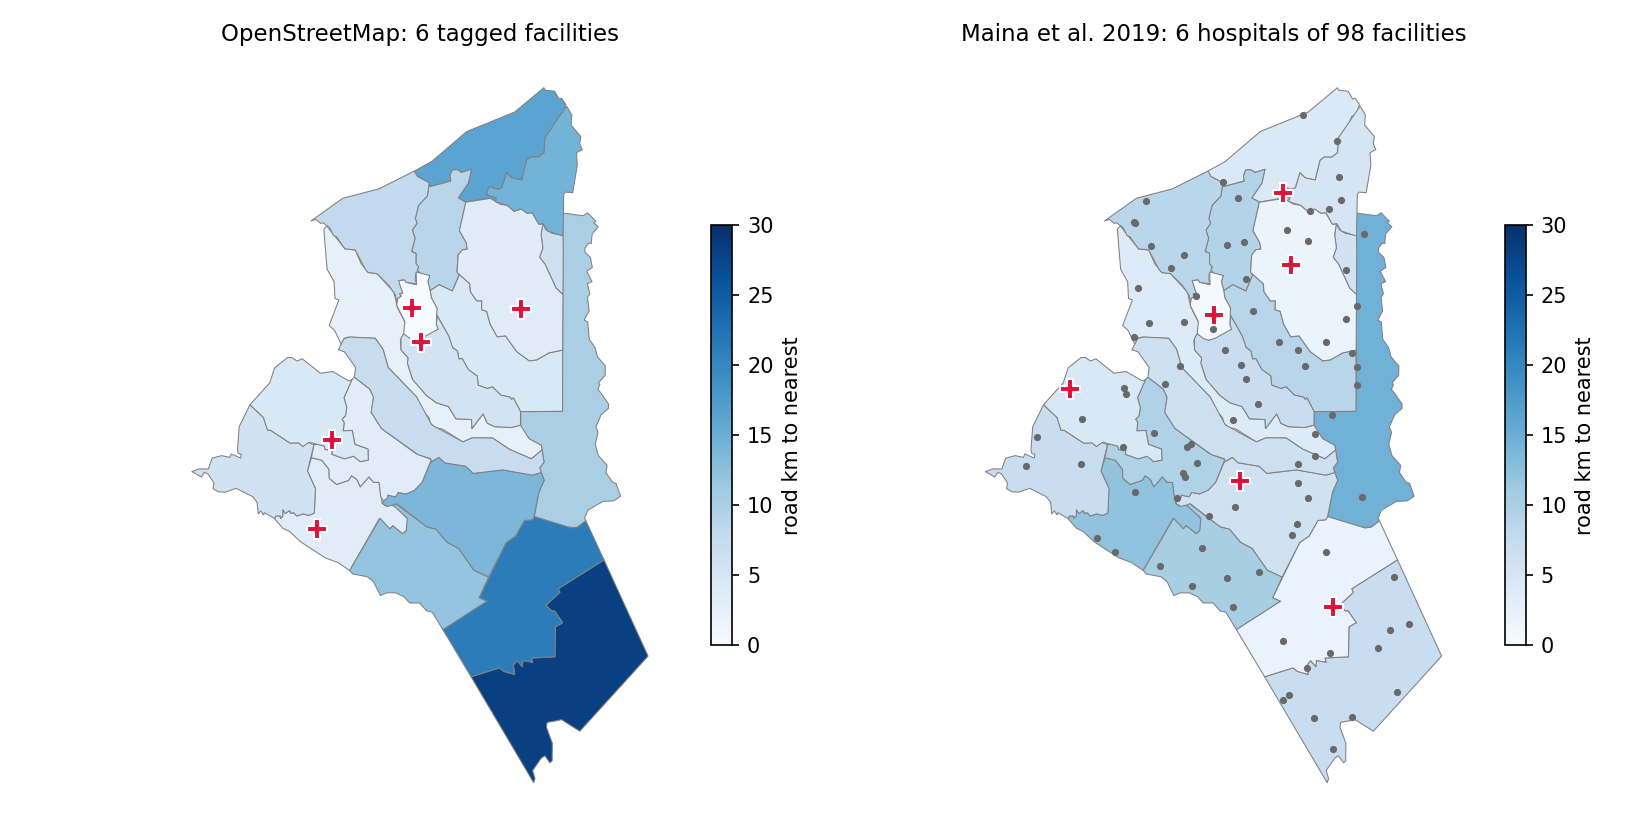
\includegraphics[width=.82\textwidth,height=.66\textheight,keepaspectratio]{figs/facilities_compare.png}\par
  \vspace{1mm}
  \small OSM tags and Maina hospital labels differ in coverage, classification and vintage. Neither comparison establishes current vaccine-storage capability.
\end{frame}

\begin{frame}{A bounded, set-based spillover}
  \[
    E_i(y)=\min\left(1,\sum_{j\ne i}e^{-\bar d_{ij}/R}y_j\right),
    \qquad \mu_i(y)=b_i(1+\gamma E_i(y)).
  \]
  \begin{itemize}
    \item Negative $\gamma$: cannibalisation. Positive $\gamma$: mobilisation.
    \item Base demand uses population, a simulated unvaccinated share and accessibility.
    \item The visited set changes turnout; visit order changes only travel.
  \end{itemize}
  \vspace{3mm}
  This simplified mechanism has no chronological patient movement or population-conservation model.
\end{frame}

\begin{frame}{Expected service includes the capacity limit}
  \[
    S_i=\min(C,\mu_i\epsilon_i),\qquad
    \epsilon_i\sim\operatorname{LogNormal}(-\sigma^2/2,\sigma).
  \]
  The noise has mean one. With $a=(\log(C/\mu)+\sigma^2/2)/\sigma$,
  \[
    h(\mu)=\mathbb E[\min(C,\mu\epsilon)]
           =\mu\Phi(a-\sigma)+C\Phi(-a).
  \]
  \begin{itemize}
    \item Train predictors of capped service, using noisy observations.
    \item Evaluate every route with this exact expectation.
    \item Optimise the known simulator expectation with a bounded interpolation error.
  \end{itemize}
\end{frame}

\begin{frame}{A deliberately informative synthetic history}
  \small
  \TrainingExample
  \vspace{3mm}
  \begin{itemize}
    \item 1500 training periods, 400 independent held-out periods.
    \item Random deployments of zero to ten wards, including zero exposure.
    \item Potential service at every ward, including unvisited wards.
    \item These displayed rows come from the actual generated training data.
  \end{itemize}
  \vspace{2mm}
  Real records introduce missing outcomes, capacity censoring and selective historical routing. They need a separate identification and validation strategy.
\end{frame}

\begin{frame}{The same predictor, two ways to plan}
  \begin{tabular}{lll}
    \toprule
    Predictor & Static policy & Embedded policy\\
    \midrule
    Linear regression & Exposure fixed at zero & Exposure depends on $y$\\[2mm]
    ReLU network & Exposure fixed at zero & Exposure depends on $y$\\
    \bottomrule
  \end{tabular}\par
  \vspace{4mm}
  \begin{itemize}
    \item Both policies use the same fitted model and training history.
    \item Predictions are clipped consistently to $[0,C]$.
    \item A historical-mean forecast is an additional static baseline.
    \item Validation uses held-out deployments, not training $R^2$.
  \end{itemize}
\end{frame}

\begin{frame}{Routing with decision-dependent service}
  \[
    \max\ \sum_i z_i-\lambda\sum_{i\ne j}d_{ij}x_{ij},\qquad
    0\le z_i\le Cy_i,\qquad z_i\le \widehat h_i.
  \]
  \begin{itemize}
    \item $y_i$ chooses serviced wards; $x_{ij}$ chooses travel arcs.
    \item An open path starts at Township; at most $K$ wards receive service.
    \item With embedding, $\widehat h_i=\max\{0,g(f_i,E_i(y))\}$ changes with the plan.
    \item The simulator benchmark approximates $h(\mu_i(y))$ from below.
  \end{itemize}
  \vspace{3mm}
  Benchmark upper bound = solver bound + at most 0.5 dose-equivalent interpolation error. Route values use the exact expectation. Complete models are in the backup slides.
\end{frame}

\begin{frame}{Environment for these results}
  \small
  \RunEnvironment
  \vspace{3mm}
  \begin{itemize}
    \item Model-building and solver times are recorded separately.
    \item Cached geography; no imported incumbent or warm start.
    \item Background load is uncontrolled and unmeasured.
    \item These are single-machine teaching results, not a runtime benchmark.
  \end{itemize}
\end{frame}

\begin{frame}{Cannibalisation: doses, distance and objective}
  \centering
  \ScenarioA
  \vspace{3mm}
  \begin{itemize}
    \item Compare static and embedded policies within each predictor.
    \item More service can require more driving. Doses/km is a different metric.
    \item The historical baseline is competitive in this synthetic setting.
  \end{itemize}
  \vspace{1mm}\small Synthetic outcomes; objective = expected doses minus one dose-equivalent per km.
\end{frame}

\begin{frame}{Mobilisation: a benefit is not guaranteed}
  \centering
  \ScenarioB
  \vspace{3mm}
  \begin{itemize}
    \item A fitted model may misrepresent decision-dependent service.
    \item Embedding does not guarantee a better decision than a careful forecast.
    \item The benchmark interval quantifies numerical uncertainty.
  \end{itemize}
  \vspace{1mm}\small Synthetic outcomes; all policies use the same capacity and road costs.
\end{frame}

\begin{frame}{The selected routes}
  \centering
  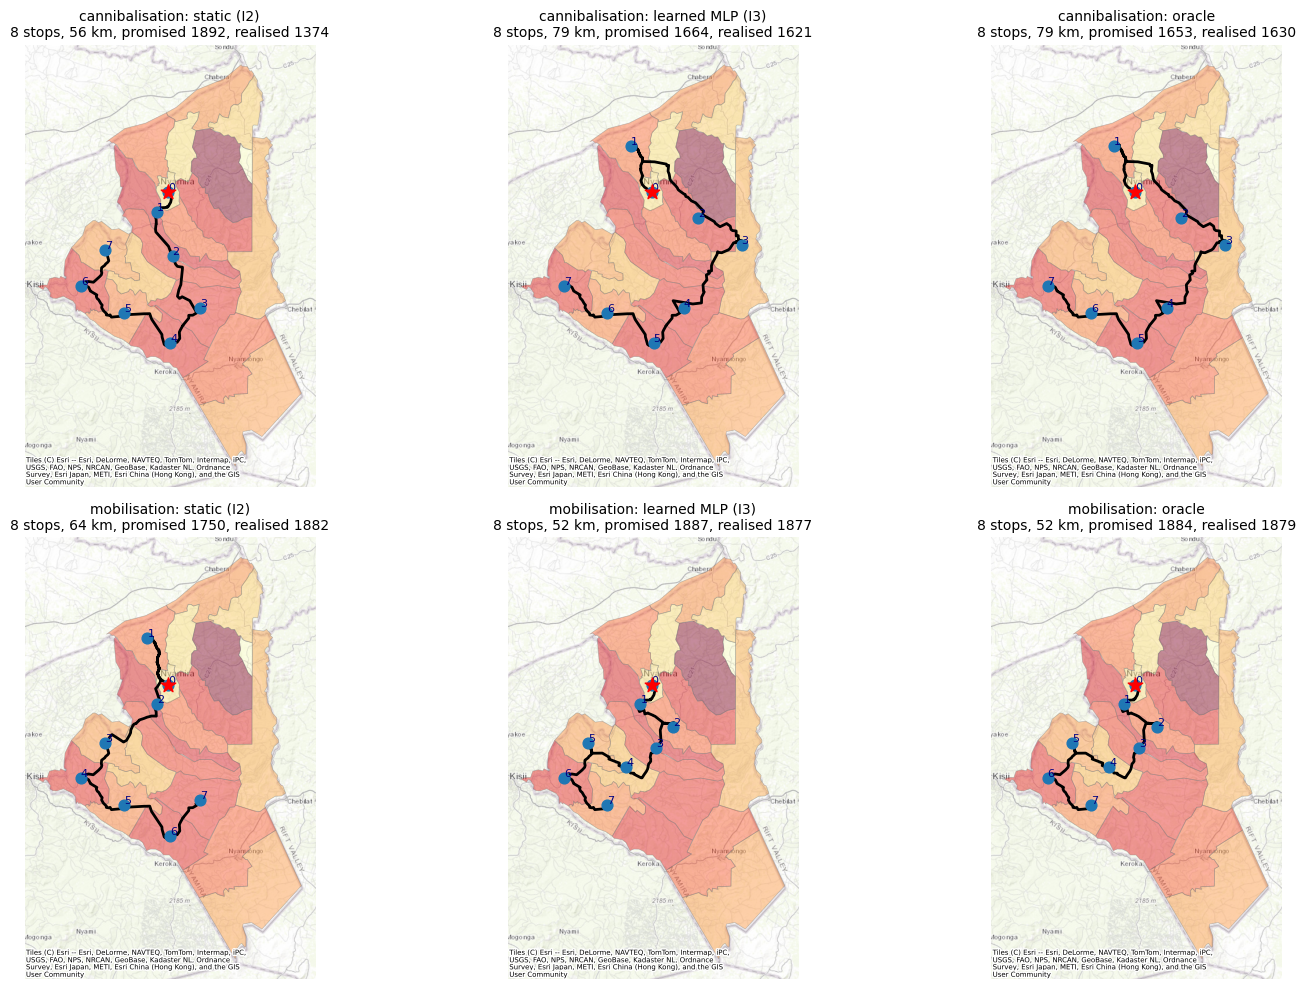
\includegraphics[width=\textwidth,height=.83\textheight,keepaspectratio]{figs/routes.png}
\end{frame}

\begin{frame}{Sensitivity to the assumed interaction}
  \centering
  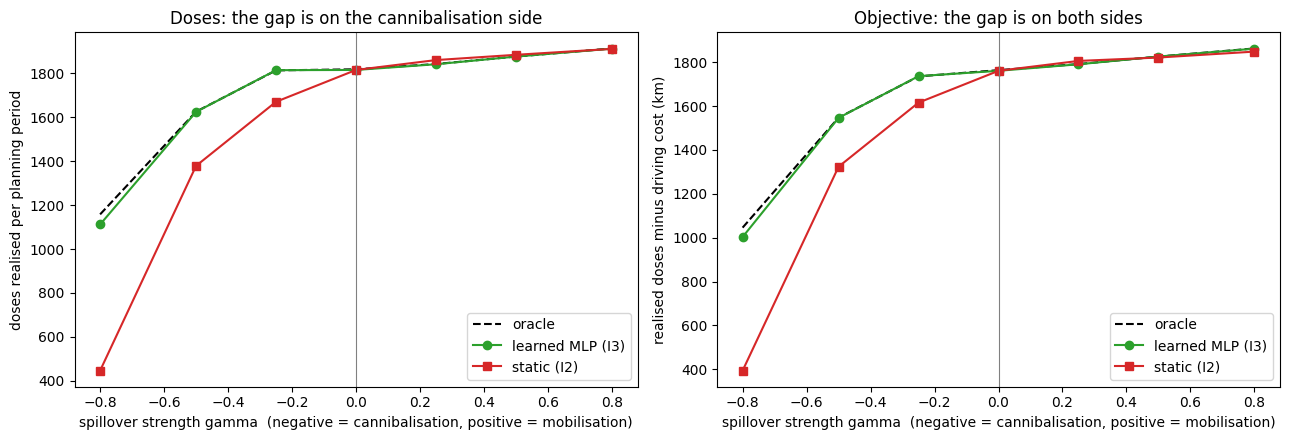
\includegraphics[width=.9\textwidth,height=.73\textheight,keepaspectratio]{figs/sweep.png}\par
  \small Each strength uses matched histories. The band includes the benchmark's solver and interpolation bounds.
\end{frame}

\begin{frame}{Live demo: a prediction before each run}
  \begin{enumerate}
    \item Change the interaction range from 10 km to 5 or 20 km.
    \item Change the stop budget from 8 to 4 or 12.
    \item Reduce the network from 8 hidden units to 2, keeping its training data fixed.
  \end{enumerate}
  \vspace{4mm}
  Predict expected doses, driving distance and their weighted objective separately.\par
  \vspace{4mm}
  The notebook also compares three independent training histories. Rerun times depend on the machine and the model; solver limits and gaps stay visible.\par
  \vspace{3mm}
  \weblink{https://colab.research.google.com/github/gromicho/mobile_clinics/blob/main/mobile_clinic_routing.ipynb}{Open the notebook in Colab}
\end{frame}

\begin{frame}{What would make this an operational study?}
  \begin{itemize}
    \item Actual service and collection locations, verified cold-chain arrangements and travel/time constraints.
    \item A defensible model of spillover, observed and censored outcomes, and historical deployment decisions.
    \item Held-out decision performance, geographic validation and programme-specific fairness requirements.
  \end{itemize}
  \vspace{4mm}
  \begin{block}{The teaching conclusion}
    Decisions can change the quantities we predict. Embedding makes that dependence explicit; its value still depends on the model, the data and the objective.
  \end{block}
  \small \weblink{https://github.com/gromicho/mobile_clinics}{Code, results, sources and slides}
\end{frame}

\pdfstringdefDisableCommands{\def\translate#1{#1}}
\appendix
\begin{frame}{Backup: model notation and inputs}
  \small
  \begin{tabular}{lp{.76\textwidth}}
    \toprule
    Symbol & Meaning\\\midrule
    $N,\ A$ & Wards; directed arcs $A=\{(i,j)\in N^2:i\ne j\}$.\\[1mm]
    $s,\ d_{ij}$ & Township depot; directed shortest-road distance in km.\\[1mm]
    $K,\ C,\ \lambda$ & Stop limit (8), capacity per stop (250), cost per km (1).\\[1mm]
    $P_i,u_i,a_i$ & Population, simulated unvaccinated share, normalised hospital distance.\\[1mm]
    $f_i,b_i$ & Features $f_i=(\log P_i,u_i,a_i)$; base demand $b_i=.02P_i u_i(.5+a_i)$.\\[1mm]
    $R,\gamma,\sigma$ & Interaction range (10 km), spillover strength ($>\!-1$), noise (.15).\\
    \bottomrule
  \end{tabular}\par\vspace{3mm}
  $x_{ij}\in\{0,1\}$ selects travel arcs; $y_i\in\{0,1\}$ selects service stops;
  $z_i\ge0$ is modelled service. Exposure and predictor outputs are continuous auxiliaries.
  \par\vspace{2mm}
  The depot receives service and counts toward $K$. Capacity is per stop; there is no total vehicle-inventory constraint.
\end{frame}

\begin{frame}{Backup: complete routing and service formulation}
  \small
  \[
  \begin{aligned}
    \max\quad &\sum\nolimits_{i\in N}z_i-\lambda\sum\nolimits_{(i,j)\in A}d_{ij}x_{ij}\\
    \text{s.t.}\quad &y_s=1,\quad \sum\nolimits_{i\ne s}x_{is}=0,\quad \sum\nolimits_i y_i\le K,\\
    &\sum\nolimits_{j\ne i}x_{ji}=y_i && i\in N\setminus\{s\},\\
    &\sum\nolimits_{j\ne i}x_{ij}\le y_i && i\in N,\\
    &\sum\nolimits_{(i,j)\in A}x_{ij}=\sum\nolimits_i y_i-1,\\
    &\sum\nolimits_{i,j\in S:i\ne j}x_{ij}\le\sum\nolimits_{i\in S}y_i-y_k
      &&\varnothing\ne S\subseteq N\setminus\{s\},\ k\in S,\\
    &0\le z_i\le Cy_i,\quad z_i\le\widehat h_i &&i\in N,\\
    &x_{ij}\in\{0,1\},\quad y_i\in\{0,1\} &&(i,j)\in A,\ i\in N.
  \end{aligned}
  \]
  \footnotesize The subtour family is added lazily. These constraints give one open path from $s$, including the one-stop route. The next slides define $\widehat h_i$ for every policy.
\end{frame}

\begin{frame}{Backup: exposure and policy-specific service}
  \small
  For embedded policies and the simulator benchmark, for every $i\in N$:
  \[
    w_{ii}=0,\quad w_{ij}=\exp\!\left(-\frac{d_{ij}+d_{ji}}{2R}\right),\quad
    r_i=\sum_jw_{ij}y_j,\quad E_i=\min\{1,r_i\}.
  \]
  Bounds: $0\le r_i\le\max_k\sum_jw_{kj}$ and $0\le E_i\le1$.
  \[
    \widehat h_i=\begin{cases}
      \max\{0,g(f_i,0)\}, &\text{static linear or MLP},\\[1mm]
      \max\{0,g(f_i,E_i)\}, &\text{embedded linear or MLP},\\[1mm]
      T^{-1}\sum_{t=1}^T S_{it}, &\text{historical mean}.
    \end{cases}
  \]
  All policies also impose $z_i\le Cy_i$. Maximising $z_i$ therefore clips service to $[0,C]$ at visited wards and gives zero at unvisited wards.
  \par\vspace{3mm}
  In the static models these service bounds are precomputed constants. The embedded models impose the min/max relations as exact general constraints.
\end{frame}

\begin{frame}{Backup: the fitted predictor inside the model}
  \small
  For input $v_i=(f_i,e_i)\in\mathbb R^4$, with $e_i=0$ (static) or $E_i$ (embedded),
  apply the fitted scaler: $t_{i\ell}=(v_{i\ell}-m_\ell)/s_\ell$, $\ell=1,\ldots,4$.
  \par\vspace{2mm}
  \textbf{Linear regression}
  \[
    q_i=\beta_0+\sum_{\ell=1}^4\beta_\ell t_{i\ell},\qquad
    \widehat h_i=\max\{0,q_i\}.
  \]
  \textbf{One-hidden-layer ReLU network (default $H=8$)}
  \[
    a_{ih}=c_h+\sum_{\ell=1}^4B_{h\ell}t_{i\ell},\quad
    v^+_{ih}=\max\{0,a_{ih}\},\qquad h=1,\ldots,H,
  \]
  \[
    q_i=c_0+\sum_{h=1}^H\alpha_h v^+_{ih},\qquad
    \widehat h_i=\max\{0,q_i\}.
  \]
  All scaler and predictor coefficients are fixed after training. Affine auxiliaries are real; ReLU and clipped outputs are nonnegative. The min/max constraints have exact mixed-integer representations in Gurobi.
\end{frame}

\begin{frame}{Backup: synthetic service and its expectation}
  \small
  For each ward and deployment, the teaching simulator specifies
  \[
    \mu_i=b_i(1+\gamma E_i),\qquad
    \epsilon_i\sim\operatorname{LogNormal}(-\sigma^2/2,\sigma),\qquad
    S_i=\min\{C,\mu_i\epsilon_i\}.
  \]
  For $\mu>0$ and $\sigma>0$, with $a=(\log(C/\mu)+\sigma^2/2)/\sigma$,
  \[
    h(\mu)=\mathbb E[\min\{C,\mu\epsilon\}]
           =\mu\Phi(a-\sigma)+C\Phi(-a).
  \]
  Here $\Phi$ is the standard normal CDF. The limiting cases are
  $h(0)=0$ and, for $\sigma=0$, $h(\mu)=\min\{C,\mu\}$.
  \par\vspace{4mm}
  The predictors are fitted to noisy capped outcomes $S_{it}$ from 1500 simulated
  periods; 400 independent periods supply validation. Every ward has a potential
  outcome in every period. Model fitting precedes routing; the routing solver does not retrain the predictor.
\end{frame}

\begin{frame}{Backup: simulator benchmark and route evaluation}
  \small
  Write $H_i(e)=h(b_i(1+\gamma e))$, using the expected capped service function.
  On each interval $[e_{i\ell},e_{i,\ell+1}]$ of a grid covering $[0,1]$, set
  \[
    a_{i\ell}=\frac{H_i(e_{i,\ell+1})-H_i(e_{i\ell})}{e_{i,\ell+1}-e_{i\ell}},
    \qquad c_{i\ell}=H_i(e_{i\ell})-a_{i\ell}e_{i\ell}.
  \]
  Keep all routing, exposure and capacity constraints. Replace the predictor bound by
  \[
    z_i\le a_{i\ell}E_i+c_{i\ell}\qquad\text{for every }i,\ell.
  \]
  Concavity makes the minimum of these lines a secant under-estimator of $H_i$.
  When $\sigma=0$, use $z_i\le b_i(1+\gamma E_i)$ together with $z_i\le Cy_i$.
  \par\vspace{2mm}
  Evaluate every returned route $(x^*,y^*)$ with the same exact expected objective:
  \[
    F(x^*,y^*)=\sum_i y_i^*h\!\left(b_i(1+\gamma E_i(y^*))\right)
              -\lambda\sum_{(i,j)\in A}d_{ij}x_{ij}^*.
  \]
\end{frame}

\begin{frame}{Backup: a bound on benchmark interpolation}
  \small
  Expected capped service is concave in exposure. For $\sigma>0$,
  \[
    \left|\frac{d^2h(b_i(1+\gamma E))}{dE^2}\right|
       \le M_i=\frac{(b_i\gamma)^2e^{\sigma^2}}{C\sigma\sqrt{2\pi}}.
  \]
  A secant over width $\Delta$ underestimates by at most $M_i\Delta^2/8$.
  Choose each ward's grid so its error is at most $\varepsilon/K$.
  \[
    \text{exact feasible route value}\ \le\ \text{optimal expected value}
      \ \le\ \text{solver bound}+\varepsilon.
  \]
  Here $\varepsilon=0.5$ dose-equivalent. Tests check the expectation against numerical integration and small routing instances against exhaustive search.
\end{frame}
